
\chapter{Generalities on image processing}\label{ch:generalities-on-image-processing}
\chead{}
\lhead{\bfseries \chaptername {\,} \thechapter }
\cfoot{\bfseries \thepage}
\rhead{}
\rhead{\bfseries Generalities on image processing}

\section{Introduction}\label{sec:introduction-ch1}
Images are one of the most important solutions that man has used to transmit and deliver knowledge and information since the dawn of humanity, in which a single image can gather a huge amount of information, Understanding the image and extracting information from the image to accomplish some works is an important area of application in digital image technology.
Modern digital technology has made it possible to manipulate images with systems that range from simple digital circuits to advanced parallel computers. The goal of this manipulation can be divided into three categories:
\begin{itemize}
        \item Image Processing\hspace{2cm} image in $\rightarrow$ image out.
        \item Image Analysis\hspace{2.4cm} image in $\rightarrow$ measurements out.
        \item Image Understanding\hspace{1.3cm} image in $\rightarrow$ high-level description out.
\end{itemize}
In this chapter, we will introduce some general concepts in the field of image processing by setting some definitions and different methods used in image processing and analyses image (image segmentation).


\section{Digital Image}\label{sec:Digital-Image}
\subsection{Definition}\label{subsec:definition}

A digital image a [m, n] described in a 2D discrete space is derived from an analog image a(x,y) in a 2D continuous space through a sampling process that is frequently referred to as digitization.
2D continuous image a(x,y) is divided into N rows and M columns.
The intersection of a row and a column is termed a pixel.
The value assigned to the integer coordinates [m,n] with $\left\{ m=0,1,2, \ldots ,M - 1 \right\}$ and $\left\{ n=0,1,2,\ldots,N - 1 \right\}$ is a[m,n].
In fact, in most cases a(x,y) which we might consider to be the physical signal that impinges on the face of a 2D sensor is actually a function of many variables including depth (z), colour ($\lambda$), and time (t).\\

        \begin{figure}[h]
                \centering
                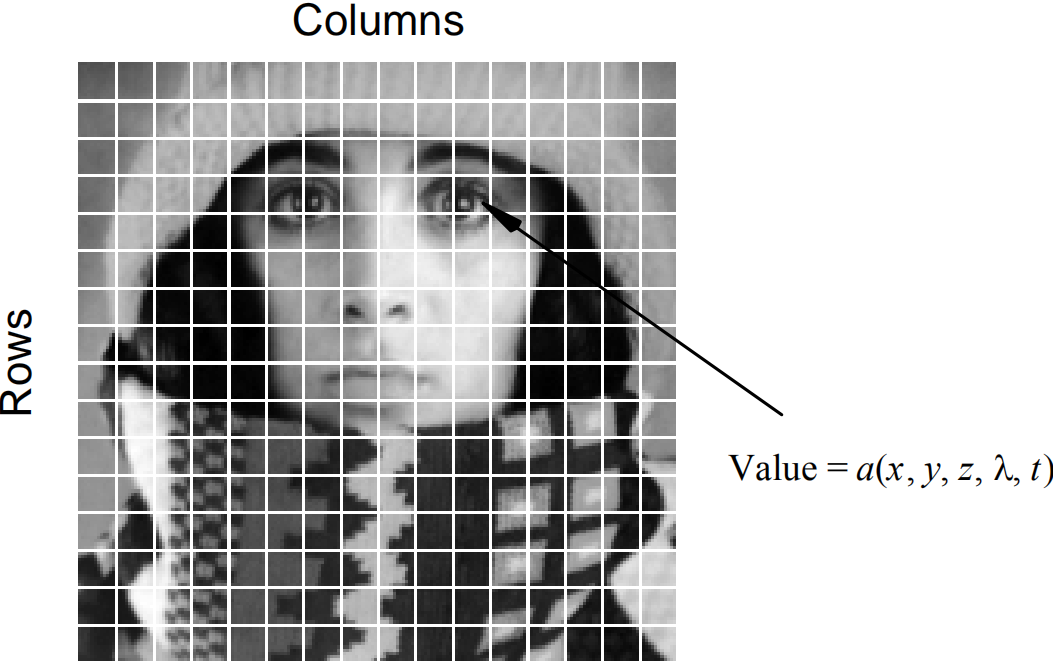
\includegraphics[width=10cm]{chapiter1/figures/degital-image.png}
                \setlength{\fboxrule}{2pt}
                \caption{Digitization of a continuous image [1].}
        \end{figure}

The image shown in Figure 1 has divided into N = 16 rows and M = 16columns.
The value assigned to every pixel is the average brightness in the pixel rounded to the nearest integer value.
The process of representing the amplitude of the 2D signal at a given coordinate as an integer value with L different grey levels is usually called amplitude quantization or simply quantization [1].

\subsection{Pixel}\label{subsec:pixel}

Pixel (or picture element) is the smallest item of information in an image.
Pixels are arranged in a 2-dimensional grid, represented using squares.
Each pixel is a sample of an original image, where more samples typically provide more-accurate representations of the original.
The intensity of each pixel is variable, in colour systems, each pixel has typically three or four components such as red, green, and blue, or cyan, magenta, yellow, and black [2].

        \begin{figure}[h]
                \centering
                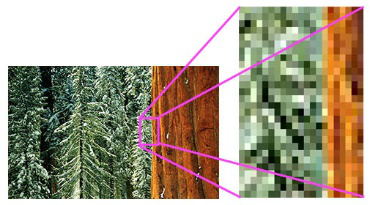
\includegraphics[width=10cm]{chapiter1/figures/pixel.png}
                \setlength{\fboxrule}{2pt}
                \caption{Pixels of part of image}
        \end{figure}

\subsection{Pixel connectivity}\label{subsec:pixel-connectivity}

Pixel connectivity is defined in terms of pixel neighbourhoods.
A normal rectangular sampling pattern producing a finite arithmetic lattice
$\left\{ (x,y) : x = 0,1, \ldots ,X-1; y = 0,1,\ldots ,Y-1 \right\}$ supporting digital
images allows us to define two types of neighbourhood surrounding a pixel [3]:

        \begin{itemize}
                \item \textbf{4-neighbourhood:} $\left\{ (x-1,y), (x,y+1), (x+1,y), (x,y-1) \right\}$ contains only the pixels above, below, to the left and to the right of the central pixel (x,y).
                \item \textbf{8-neighbourhood:} adds to the 4-neighbourhood four diagonal neighbours: $\left\{ (x-1,y-1), (x-1,y+1), (x+1,y+1), (x+1,y-1) \right\}$ .
        \end{itemize}

        \begin{figure}[h]
                \centering
                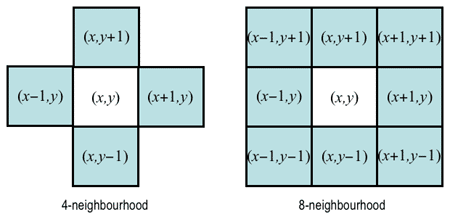
\includegraphics[width=6cm]{chapiter1/figures/neighbour.png}
                \setlength{\fboxrule}{2pt}
                \caption{pixel neighborhood}
        \end{figure}

\section{Type of Digital Image}\label{sec:type-of-digital-image}

For photographic purposes, there are two important types of digital image colour and grey-scale images (black and white).
Colour images contain coloured pixels and grey-scale images are made of pixels in different shades of grey.

\subsection{Colour Image}

Colour image is made up of pixels each of which holds three numbers corresponding to the red, green, and blue levels of the
image at a particular location. Red, green, and blue (sometimes referred to as RGB) are the primary colours for mixing
light these called additive primary colours which  are different from the subtractive primary colours used for mixing
paints (cyan, magenta, and yellow). Any colour can be created by mixing the correct amounts of red, green, and blue light.
Assuming 256 levels for each primary, each colour pixel can be stored in three bytes (24 bits) of memory this corresponds to $2^{24}=16777216$ different colours [4].\\
However, it is computationally expensive and often not necessary to use the full 24-bit image to store the colour for each pixel.
Therefore, the colour for each pixel is often encoded in a single byte, resulting in an 8-bit colour image. The process of reducing
the colour representation from 24-bits to 8-bits, known as colour quantization, restricts the number of possible colours to 256.
However, there is normally no visible difference between a 24-colour image and the same image displayed with 8 bits. An 8-bit colour
images are based on colour maps, which look-up tables are taking the 8-bit pixel value as index and providing an output value for each colour [5].

        \begin{itemize}
                \item Each pixel is represented by three bytes (e.g RGB).
                \item 640 x 480 24-bit color image would require 921.6 KB of storage.
        \end{itemize}

        \vspace{4cm}

        \begin{figure}[h]
                \centering
                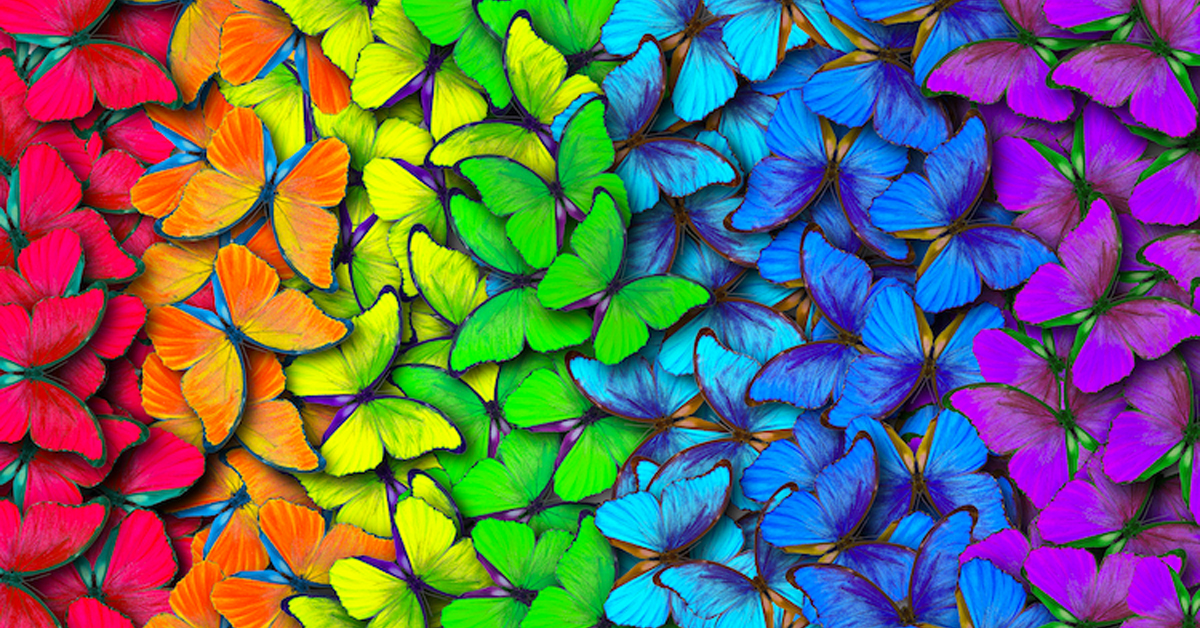
\includegraphics[width=10cm]{chapiter1/figures/color-image.jpg}
                \setlength{\fboxrule}{2pt}
                \caption{Color Image}
        \end{figure}



\subsection{Grey-Scale Image}
The grayscale image adds a colour depth between black and white in the binary image to form a grayscale image.
4Such images are usually displayed as grayscales from the darkest black to the brightest white, and each colour
depth is called a grayscale, usually denoted by L. In grayscale images, pixels can take integer values between 0 and L-1 [6].

        \begin{itemize}
                \item Each pixel is usually stored as a byte (value between 0 and 255).
                \item A 640 x 480 greyscale image requires over 300 KB of storage.
        \end{itemize}
\textbf{Note:}  that for grey scale images will use three times less memory than a colour version.

        \begin{figure}[h]
                \centering
                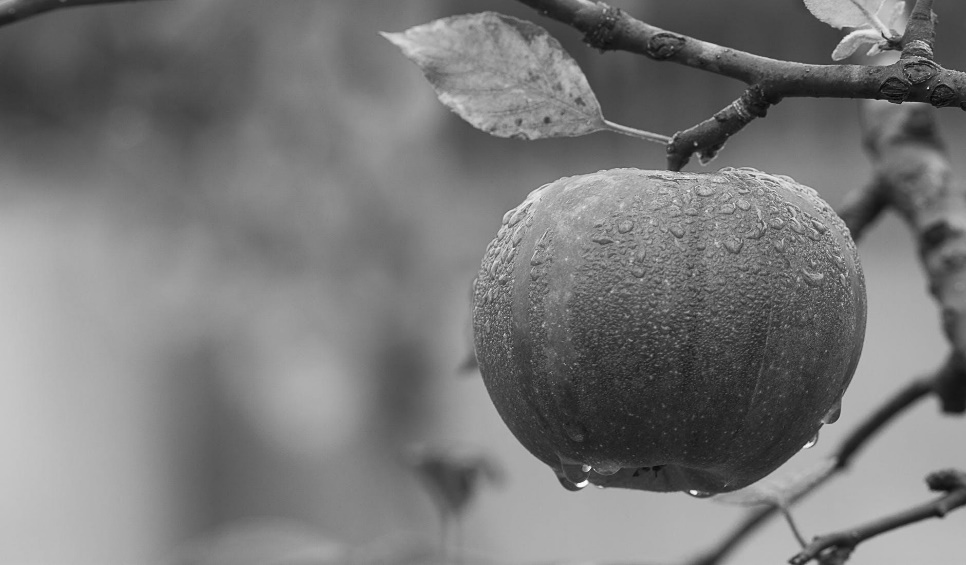
\includegraphics[width=10cm]{chapiter1/figures/grey-scal.png}
                \setlength{\fboxrule}{2pt}
                \caption{Grey-Scale Image}
        \end{figure}

To convert from a color image to gray scale image there is two method [7]:

        \begin{enumerate}
                \item \textbf{Average Method :} \\
                The Average method takes the average value of Red, Green, and Blue as the greyscale value:
                \begin{equation}
                        GreyScale = (R + G + B) /3\label{eq:equation}
                \end{equation}
                The average method is simple but does not work as well as expected.
                The reason being that human eyeballs react differently to RGB.
                Eyes are most sensitive to green light, less sensitive to red light,
                and the least sensitive to blue light. Therefore, the three colours should have
                different weights in the distribution. That brings us to the weighted method.
                \item \textbf{Average Method :} \\
                The weighted method, also called luminosity method, weighs Red,
                Green and Blue according to their wavelengths the improved formula is as follows :
                \begin{equation}
                        GrayScale = 0.299R + 0.587G + 0.114B\label{eq:equation2}
                \end{equation}
                As it shown in figure 1.6 the different between two-method one the weighted method better than the average method.
                \begin{figure}[h]
                        \centering
                        \begin{subfigure}[b]{0.3\textwidth}
                                \centering
                                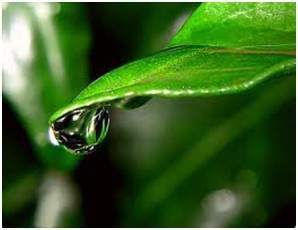
\includegraphics[width=\textwidth]{chapiter1/figures/original-grey.png}
                                \caption{Original image}
                        \end{subfigure}
                        \hfill
                        \begin{subfigure}[b]{0.3\textwidth}
                                \centering
                                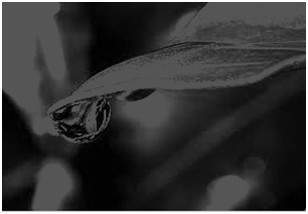
\includegraphics[width=\textwidth]{chapiter1/figures/avarage-grey.png}
                                \caption{Average Method}
                        \end{subfigure}
                        \hfill
                        \begin{subfigure}[b]{0.3\textwidth}
                                \centering
                                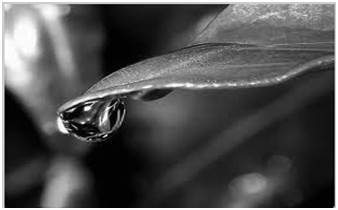
\includegraphics[width=\textwidth]{chapiter1/figures/withed-grey.png}
                                \caption{The Weighted Method}
                        \end{subfigure}
                        \caption{The GreyScal Convertion }
                \end{figure}
        \end{enumerate}
\subsection{Binary image}
Binary images are the simplest type of images and can take on two values,
typically black and white, or (0) and (1).
A binary image is referred to as a 1 bit/pixel image because it takes only 1
binary digit to represent each pixel.
These types of images are most frequently in computer vision application where the
only information required for the task is general shapes, or outlines information.
For example, to position a robotics gripper to grasp an object or in optical character
recognition (OCR). Binary images are often created from gay-scale images via a threshold
value is turned white (1), and those below it are turned black (0) [8].

        \begin{itemize}
                \item Each pixel is stored as a single bit (0 or 1).
                \item A 640 x 480 monochrome image requires 37.5 KB of storage.
        \end{itemize}

        \begin{figure}[h]
                \centering
                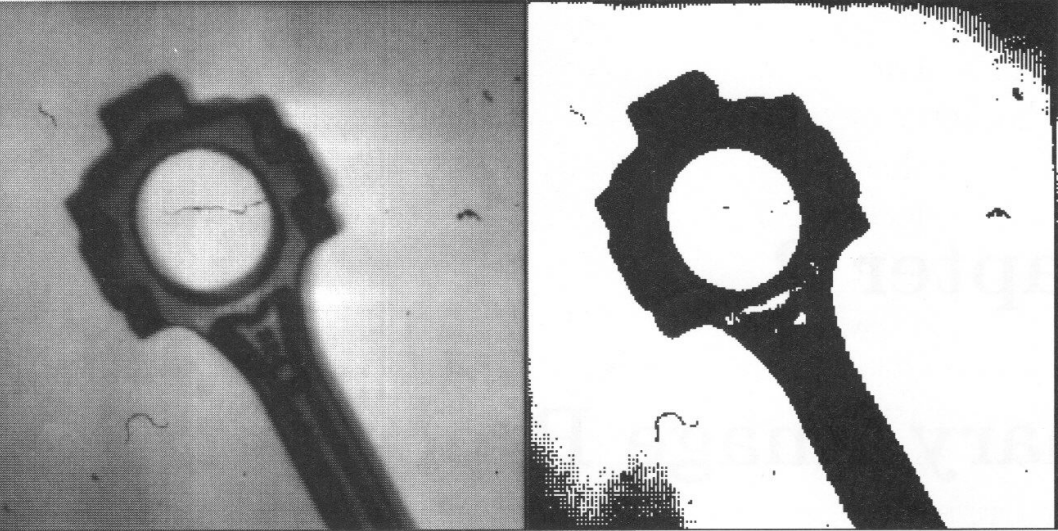
\includegraphics[width=10cm]{chapiter1/figures/binaire.png}
                \setlength{\fboxrule}{2pt}
                \caption{ A gray level image and its corresponding binary image}
        \end{figure}

\section{Image Enhancement Method}\label{sec:image-enhancement-method}
Image enhancement is improving the interpretability or perception of information in images
for human viewers and providing `better' input for other automated image processing techniques.
The principal objective of image enhancement is to modify attributes of an image to make it
more suitable for a given task and a specific observer.

\subsection{Simple intensity transformation}
\subsubsection{Image negatives}
Negatives of digital images are useful in numerous applications,
such as displaying medical images and photographing a screen with monochrome positive
film with the idea of using the resulting negatives as normal slides [9].Transform function is given as Eq(3).

        \begin{equation}
                g(x,y) = L - f(x,y)
        \end{equation}
with L $\rightarrow$ the max intensity.

        \begin{figure}[h]
                \centering
                \begin{subfigure}[b]{0.46\textwidth}
                        \centering
                        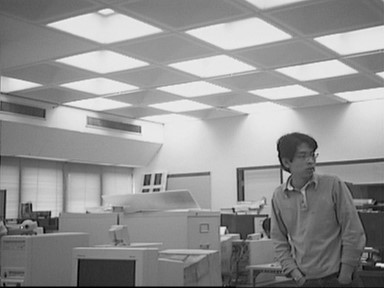
\includegraphics[width=\textwidth]{chapiter1/figures/original-negative-image.jpg}
                        \caption{Original image}
                \end{subfigure}
                \hfill
                \begin{subfigure}[b]{0.46\textwidth}
                        \centering
                        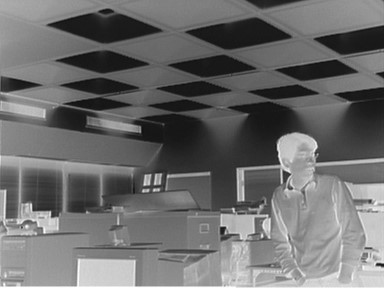
\includegraphics[width=\textwidth]{chapiter1/figures/negative-image.jpg}
                        \caption{Negative image}
                \end{subfigure}
                \caption{A gray level image and its corresponding negative image}
        \end{figure}

\subsubsection{Contrast stretching}
Low-contrast images can result from poor illumination, lack of dynamic range in the image sensor,
or even wrong setting of a lens aperture during image acquisition.\\
The idea behind contrast stretching is to increase the dynamic range of the grey levels in the image being processed [10].\\
Figure (1.9) shows a typical transformation function used for Contrast Stretching [11].

        \begin{figure}[h]
                \centering
                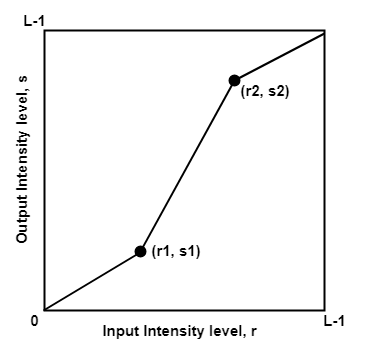
\includegraphics[width=7cm]{chapiter1/figures/linear_Transform.png}
                \setlength{\fboxrule}{2pt}
                \caption{transformation function used for Contrast Stretching [11]}
        \end{figure}

By changing the location of points (r1, s1) and (r2, s2), we can control the shape of the transformation function:
        \begin{enumerate}
                \item When r1 =s1 and r2=s2, transformation becomes a \textbf{Linear function}.
                \item When r1=r2, s1=0 and s2=L-1, transformation becomes a \textbf{thresholding function}.
                \item When (r1, s1) = (rmin, 0) and (r2, s2) = (rmax, L-1), this is known as \textbf{Min-Max Stretching}.
                \item 4.When (r1, s1) = (rmin+ c, 0) and (r2, s2) = (rmax – c, L-1), this is known as \textbf{Percentile Stretching}.
        \end{enumerate}

        \begin{figure}[h]
                \centering
                \begin{subfigure}[b]{0.46\textwidth}
                        \centering
                        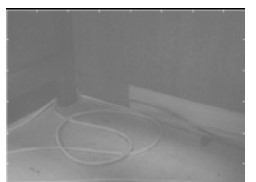
\includegraphics[width=\textwidth]{chapiter1/figures/constrat-ori.jpg}
                        \caption{Original image}
                \end{subfigure}
                \hfill
                \begin{subfigure}[b]{0.46\textwidth}
                        \centering
                        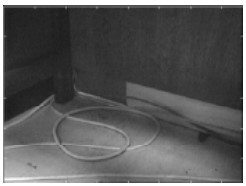
\includegraphics[width=\textwidth]{chapiter1/figures/constart-processed.jpg}
                        \caption{Processed image}
                \end{subfigure}
                \caption{A gray level image Contrast stretching}
        \end{figure}

\subsubsection{Compression of dynamic range}
Sometimes the dynamic range of a processed image far exceeds the capability of the display device,
in which case only the brightest parts of the images are visible on the display screen.
An effective way to compress the dynamic range ofpixel values is to perform the following intensity transformation function Eq(1.4):
        \begin{equation}
                s = c * log(1+|r|)
        \end{equation}
Where is a scaling constant, and the logarithm function performs the desired compression [12].

        \begin{figure}[h]
                \centering
                \begin{subfigure}[b]{0.46\textwidth}
                        \centering
                        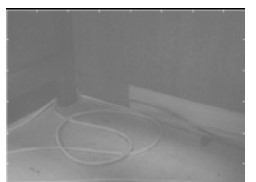
\includegraphics[width=\textwidth]{chapiter1/figures/constrat-ori.jpg}
                        \caption{Original image}
                \end{subfigure}
                \hfill
                \begin{subfigure}[b]{0.46\textwidth}
                        \centering
                        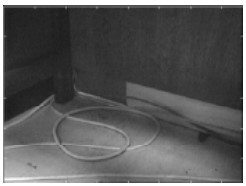
\includegraphics[width=\textwidth]{chapiter1/figures/constart-processed.jpg}
                        \caption{Processed image}
                \end{subfigure}
                \caption{Compression of dynamic range of gray level image}
        \end{figure}
        \vspace{2cm}
\subsection{Histogram processing}
Histogram processing is used in image enhancement the information inherent in histogram can also use in
other image processing application such as image segmentation and image compression. A histogram simply
plots the frequency at which each grey-level occurs from 0 (black) to 255 (white).\\
Histogram processing should be the initial step in reprocessing. To produce a much better image histogram
equalization and histogram specification (matching) are two methods widely used to modify the histogram of an image.\\
Histogram represents the frequency of occurrence of allgrey-level in the image, that means it tell
us how the values of individual pixel in an image are distributed.
Histogram is given as~\ref{eq:5}.

        \begin{equation}
                (r_k) = n_k/N\label{eq:5}
        \end{equation}

Where $r_k$ and $n_k$ are intensity level and number of pixels in image with intensity $r_k$ Respectively[13].

        \begin{figure}[h]
                \centering
                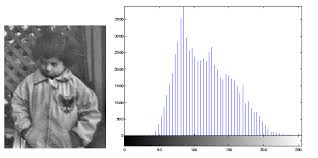
\includegraphics[width=12cm]{chapiter1/figures/image-and-hist.png}
                \setlength{\fboxrule}{2pt}
                \caption{A gray level image and its corresponding histogram [14]}
        \end{figure}

        \vspace{2cm}

\subsubsection{Histogram equalization}
Histogram equalization is a common technique for enhancing the appearance of images.
Suppose we have animate which is predominantly dark. Then its histogram would be skewed
towards the lower end of the grey scale and all the image detail is compressed into the
dark end of the histogram. If we could `stretch out' the grey levels at the dark end to
produce a more uniformly distributed histogram then the image would become much clearer.\\
Histogram equalization stretches the histogram across the entire spectrum of pixels (0 - 255).
It increases the contrast of images for the finality of human inspection and can be applied
to normalize illumination variations in image understanding problems. Histogram equalization
is one of the operations that can be applied to obtain new images based on histogram specification
or modification. Histogram equalization is considered a global technique. This process is quite
simple and for each brightness level j in the original image, the new pixel level value (k)
is calculated as given in \ref{eq:6} Where the sum counts the number of pixels in the image with
brightness equal to or less than j, and T is the total number of pixels.

        \begin{equation}
                \sum_{i = 0}^{j} \frac{N_i}{T}\label{eq:6}
        \end{equation}

The main purpose of histogram equalization is to find grey level transformation function T
to transform image f such that the histogram of T (f) is "equalized" [13].

        \begin{figure}[h]
                \centering
                \begin{subfigure}[b]{0.3\textwidth}
                        \centering
                        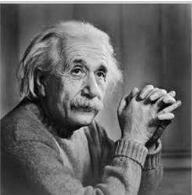
\includegraphics[width=\textwidth]{chapiter1/figures/equa-processed-hist.png}
                        \caption{Original image}
                \end{subfigure}
                \hfill
                \begin{subfigure}[b]{0.5\textwidth}
                        \centering
                        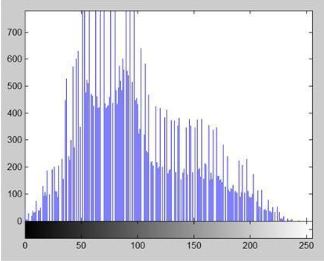
\includegraphics[width=\textwidth]{chapiter1/figures/equa-original-image.png}
                        \caption{Original Histogram}
                \end{subfigure}
                \hfill
                \begin{subfigure}[b]{0.3\textwidth}
                        \centering
                        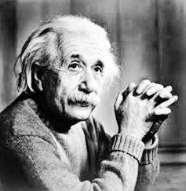
\includegraphics[width=\textwidth]{chapiter1/figures/equa-processed-image.png}
                        \caption{image Processed}
                \end{subfigure}
                \hfill
                \begin{subfigure}[b]{0.5\textwidth}
                        \centering
                        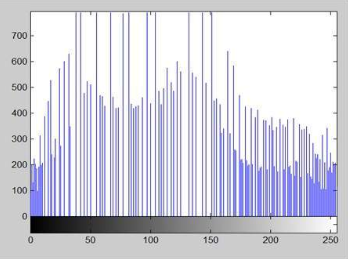
\includegraphics[width=\textwidth]{chapiter1/figures/equa-original-hist.png}
                        \caption{Equalized histogram}
                \end{subfigure}
                \caption{A grey-level image and its corresponding histogram,and its equalized histogram and thenew image corresponding}
        \end{figure}

\subsubsection{Histogram Matching}
While the goal of histogram equalization is to produce an output image that has flattened histogram, the goal
of histogram matching is to take an input image and generate an output image that is based upon the shape of a
specific (or reference) histogram. Histogram matching is also known as histogram specification.Histogram equalization
is considered as a special case of histogram matchingin which we want to force an image to have a uniform histogram
(rather than just any shape as is the case for histogram matching) [15].\\
After we get the enhanced image, we can analysing this image and extract the information from it. So now we talk
about the method and technique of analysing image (image segmentation).

\section{Image Segmentation}
\subsection{Definition}
Image segmentation is typically used to locate objects and boundaries (lines, curves, etc.) in images.
More precisely, image segmentation is the process of assigning a label to every pixel in an image such
that pixels with the same label share certain visual characteristics. The result of image segmentation is
a set of segments that collectively cover the entire image, or a set ofcontours extracted from the image.
Each of the pixels in a region are similar with respect to somecharacteristic or computed property,
such as color, intensity, or texture [1].\\
In computer vision,image processing is any form of signal processing for which the input is an image,
such asphotographs or frames of videos. The output of image processing can be either an image or a set
of characteristics or parameters related to image. Also, segmentation refers to the process ofpartitioning
a digital image into multiple segments (sets of pixels, also known as super pixels) [16].
\subsection{Goal of segmentation}
The goal of segmentation is to simplify and change the representation of an image into something that is
more meaningful and easier to analyse. Image segmentation is typically used to locate objects and boundaries in image [17].
\subsection{Image segmentation approaches}
From the international image segmentation method, the specific operation of the process ofsegmentation method is very 
diverse and complex, andthere is no recognized a unified standard. We discusses the above five methods.
\subsubsection{Region-based Segmentation}
        \begin{enumerate}{\Alph{enumi}}
                \item \textbf{Threshold Segmentation}\\
                Threshold segmentation is the simplest method of image segmentation and one of the
                most common parallel segmentation methods. It is a common segmentation algorithm,
                which directly divides the image grey scale information processing based on the grey
                value of different targets. Threshold segmentationcan be divided into local threshold
                method and globalthreshold method. The global threshold method dividesthe image into
                two regions of the target and the background by a single threshold. The local thresholdmethod
                needs to select multiple segmentation thresholds and divides the image into multiple target
                regionsand backgrounds by multiple thresholds.\\
                The most commonly used threshold segmentation algorithm is the largest interclass variance method,
                which selects a globally optimal threshold bymaximizing the variance between classes.
                In additionto this, there are entropy-based threshold segmentationmethod, minimum error method,
                co-occurrence matrixmethod, moment preserving method, simple statisticalmethod, probability
                relaxation method, fuzzy set method and threshold methods combined with othermethods.\\
                The advantage of the threshold method is that thecalculation is simple and the operation
                speed is faster.In particular, when the target and the background havehigh contrast,
                the segmentation effect can be obtained.The disadvantage is that it is difficult to obtain
                accurateresults for image segmentation problems where there is no significant grey scale
                difference or a large overlap of the grey scale values in the image. Since it only takes into
                account the grey information of the image without considering the spatial information of the image,
                it is sensitive to noise and grayscale unevenness,leading it often combined with other methods [18].
                \item \textbf{Regional Growth Segmentation}\\
                The regional growth method is a typical serial region segmentation algorithm, and its basic idea
                is tohave similar properties of the pixels together to form aregion. The method requires first
                selecting a seedpixel, and then merging the similar pixels around theseed pixel into the region
                where the seed pixel is located.\\
                \vspace{1cm}
                \begin{figure}[h]
                        \centering
                        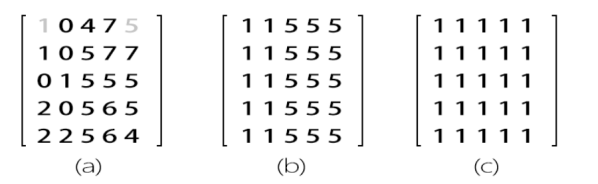
\includegraphics[width=12cm]{chapiter1/figures/regional.png}
                        \setlength{\fboxrule}{2pt}
                        \caption{Examples of regional growth}
                \end{figure}

                Figure 13 shows an example of a known seed point for region growing.
                Figure 13 (a) shows the need to split the image. There are known two seed pixels
                (marked as grey squares) which are prepared for regional growth. The criterion used here is
                that if the absolute value of the gray value difference between the pixel and the seed pixel
                is considered to be less than a certain threshold T, the pixel is included in the region where
                the seed pixel is located. Figure 1 (b) shows the regional growth results at T = 3,
                and the whole plot is well divided into two regions. Figure 1 (c) shows the results of
                the region growth at T = 6 and the whole plot is in an area. Thus the choice of threshold is very important.\\
                The advantage of regional growth is that it usually separates the connected regions with the
                samecharacteristics and provides good boundary information and segmentation results. The idea of regionalgrowth
                is simple and requires only a few seed points tocomplete. And the growth criteria in the growing process
                can be freely specified. Finally, it can pick multiple criteria at the same time. The disadvantage is thatthe
                computational cost is large. Also the noise andgrayscale unevenness can lead to voids and over division.
                The last is the shadow effect on the image is of the not very good [18].
        \end{enumerate}

\subsubsection{Edge Detection Segmentation}
The edge of the object is in the form of discontinuous local features of the image, that is,
the most significant part of the image changes in local brightness, such as grey value of the mutation,
colour mutation, texture changes and so on. The use of discontinuities todetect the edge, so as to achieve the purpose of imagesegmentation.\\
There is always a grey edge between two adjacent regions with different grey values in the image,and there is a
case where the grey value is not continuous. This discontinuity can often be detected using derivative operations,
and derivatives can be calculatedusing differential operators. Parallel edge detectionis often done by means of a spatial
domain differentialoperator to perform image segmentation by convoluting its template and image. Parallel edge detection
isgenerally used as a method of image pre-processing.The widely first-order differential operators are Prewitt-operator,
Roberts operator and Sobel operator. Thesecond-order differential operator has nonlinear operators such as Laplacian,
Kirsch operator and Wallis operator [18].\\

        \begin{enumerate}{\Alph{enumi}}
                \item \textbf{Sobel Operator} \\
                The Sobel operator is mainly used for edge detection, and it is technically a discrete differential
                operator used to calculate the approximation of the gradientof the image luminance function.
                The Sobel operator is a typical edge detection operator based on the first derivative.
                As a result of the operator in the introductionof a similar local average operation,
                so the noise has asmoth effect, and can effectively eliminate the impactof noise.
                The influence of the Sobel operator on the position of the pixel is weighted, which is better
                than thePrewitt operator and the Roberts operator.\\
                The Sobel operator consists of two sets of 3x3matrices, which are transverse and longitudinal templates,
                and are plotted with the image plane, respectively, to obtain the difference between the horizontaland
                the longitudinal difference. In actual use, the following two templates are used to detect the edges of theimage [18].
                        \begin{equation}
                                G_x =
                                \begin{bmatrix}
                                        -1 & 0 & 1 \\
                                        -2 & 0 & 2 \\
                                        -1 & 0 & 1
                                \end{bmatrix}
                                \hspace{2cm}
                                G_y =
                                \begin{bmatrix}
                                        1 & 2 & 1 \\
                                        0 & 0 & 0 \\
                                        -1 & -2 & -1
                                \end{bmatrix}
                        \end{equation}
                The horizontal and vertical gradient approximations of each pixel of the image can be combined
                tocalculate the size of the gradient using the following :
                        \begin{equation}
                                G = \sqrt[2]{G^{2}_{x} + G^{2}_{y}}
                        \end{equation}
                \item \textbf{Laplacian Operator} \\
                Laplace operator is an isotropic operator, second-order differential operator.
                It is more appropriate whenit is only concerned with the position of the edge regardless of
                the pixel grey scale difference around it.The Laplace operator's response to isolated pixels
                isstronger than the edge or line, and therefore appliesonly to noise-free images.
                In the presence of noise, theLaplacian operator needs to perform low-pass filteringbefore
                detecting the edge. Therefore, the usual segmentation algorithm combines theLaplacian operator
                withthe smoothing operator to generate a new template.
                Laplacian operator is also the simplest isotropic differential operator with rotational invariance.
                The Laplace transform of a two-dimensional image function isan isotropic second derivative,
                which is more suitablefor digital image processing, and the pull operator isexpressed as a discrete Eq(8):
                        \begin{equation}
                                \nabla^{2} f = \frac{\sigma^2 f}{\sigma x^2 } + \frac{\sigma^2 f}{\sigma y^2 }
                        \end{equation}
                In addition, the Laplace operator can also be expressed in the form of a template.
               \begin{center}
                       $
                       \begin{bmatrix}
                               0 & 1 & 0 \\
                               1 & -4 & 1 \\
                               0 & 1 & 0
                       \end{bmatrix}
                       $
               \end{center}
                The Laplacian operator is used to improve theblurring effect due to the blurring effect,
                since it conforms to the descent model. Diffusion effect is often occurring in the imaging process [18].
        \end{enumerate}
For contours extraction, some methods manipulate a shape encompassing the object to extract and move it from an initial
position to a final position corresponding to the target object. This approach is active contours.
\section{Conclusion}
In this chapter, we have presented some basic concepts on digital imaging.
Image segmentation is the basis of any vision system and is intended to provide a description of the objects in the image.
In the following chapter, we will discuss an edge-based segmentation method, called active contours.